\chapter{Results}
\label{chapter3}

\section{Evaluation Strategy}

As outlined in the introduction, the focus of this report is on showing how PBS produces more photorealistic images than Blinn-Phong shading. This is fulfilled by highlighting physical phenomena that are modelled more accurately in frames rendered using PBS, than in frames rendered using Blinn-Phong shading. Two such physical phenomena are identified below, and subsequent comparisons performed for each using the application developed.

The first phenomena is the Fresnel effect. Mentioned in section \ref{FresnelReflectance}, the Fresnel effect is the observation that a surface becomes more specular at glancing incident light angles. Faul shows that the Fresnel effect is a key contributor to the appearance of specular materials~\cite{FaulInfluenceOfFresnelEffect}. This suggests that the realism of a shading model is influenced by the degree to which it models the impact of the Fresnel effect. Therefore, it forms a suitable candidate for comparison. In an effort to further build on Faul's investigation, comparing the presence of the Fresnel effect is done by considering the impact it has on the appearance of diffuse materials, rather than specular.

The second physical phenomena is the way in which light intensity determines the appearance of an object. In the real world, light sources have an output power which defines how intense they are. Given a light source of a varying power, a comparison is performed between the two shading models to ascertain how accurately they depict how the power influences the appearance of an object.

The evaluation is also supplemented with an analysis of frame times. This assesses whether the implemented shading models are indeed sufficiently performant to be used in real time rendering.

\section{Fresnel Effect Comparison}

\subsection{Testing Method}

Testing a shading model's ability to capture the Fresnel effect could be done using a single point light that is incident to an xz-aligned plane. From a constant viewpoint, the point light could then be moved over the plane so as to vary the incident light angle. From that viewpoint, the amount of specular reflection could be observed. 

However, the test given here is instead performed by keeping the position of the point light constant, and varying the viewing angle (which is also given in respect to the surface normal). The effect of varying the viewing angle is to vary \begin{math}\vect{v}\end{math}, and thus also vary \begin{math}\vect{h}\end{math}; varying \begin{math}\vect{h}\end{math} is equivalent to varying the normals of the microfacets that contribute to the specular reflection; varing the normals has the effect of varying the incident light angle on those microfacets. Although this sequence of implications is certainly complex, carrying out the test in this manner is simpler than the alternative approach given above. Shirley et al present a case study that captures the Fresnel effect by also varying the viewing angle~\cite{PractitionersReflectionModels}. Moreover, as Figure \ref{fig:FresnelRealLife} shows, this testing approach is justified by conducting observations of the real world: the Fresnel effect causes surfaces to appear more specular at glancing viewing angles.

For the tests, two scenes were created. One for the Blinn-Phong renderer, and another for the physically based renderer. Each scene is arranged in the same manner. A diffuse wooden floor is situated at the origin, and a point light is placed just above it. Four viewing angles are considered, \begin{math}0^{\circ}\end{math}, \begin{math}40^{\circ}\end{math}, \begin{math}65^{\circ}\end{math} and \begin{math}80^{\circ}\end{math}. For each of these angles, the outputted frames of the two renderers are sampled. A shading model that captures the Fresnel effect is expected to render the floor with greater specularity as the viewing angle increases (becomes more glancing).

\begin{figure}[h]
	\centering
	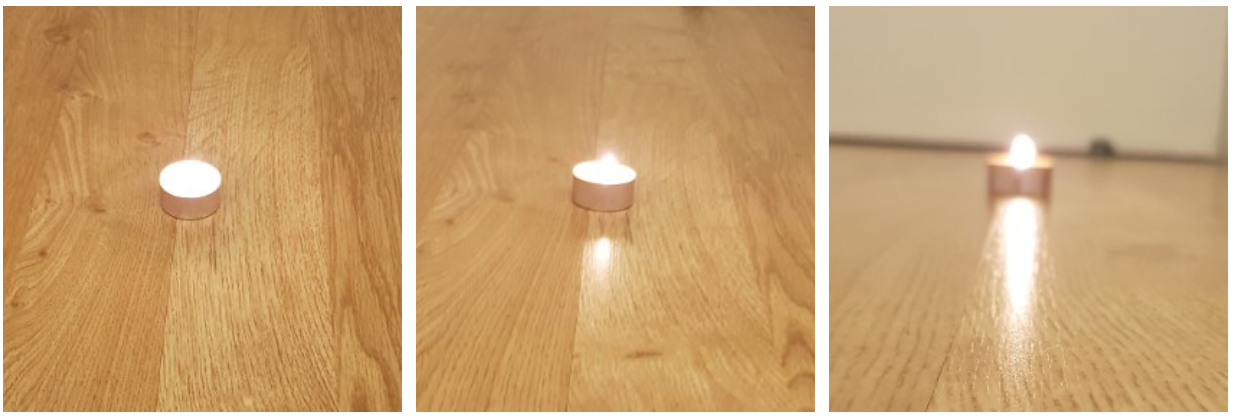
\includegraphics[width=12cm]{FresnelRealLife}
	\caption{The Fresnel effect can be observed in the real world by varying the viewing angle. Taken from~\cite{MarkusLecture}.}
	\label{fig:FresnelRealLife}
\end{figure}

\subsection{Results}

The sampled frames for the two shading models are given in Figure \ref{fig:FresnelResults}.

\begin{figure}[h]
	\centering
	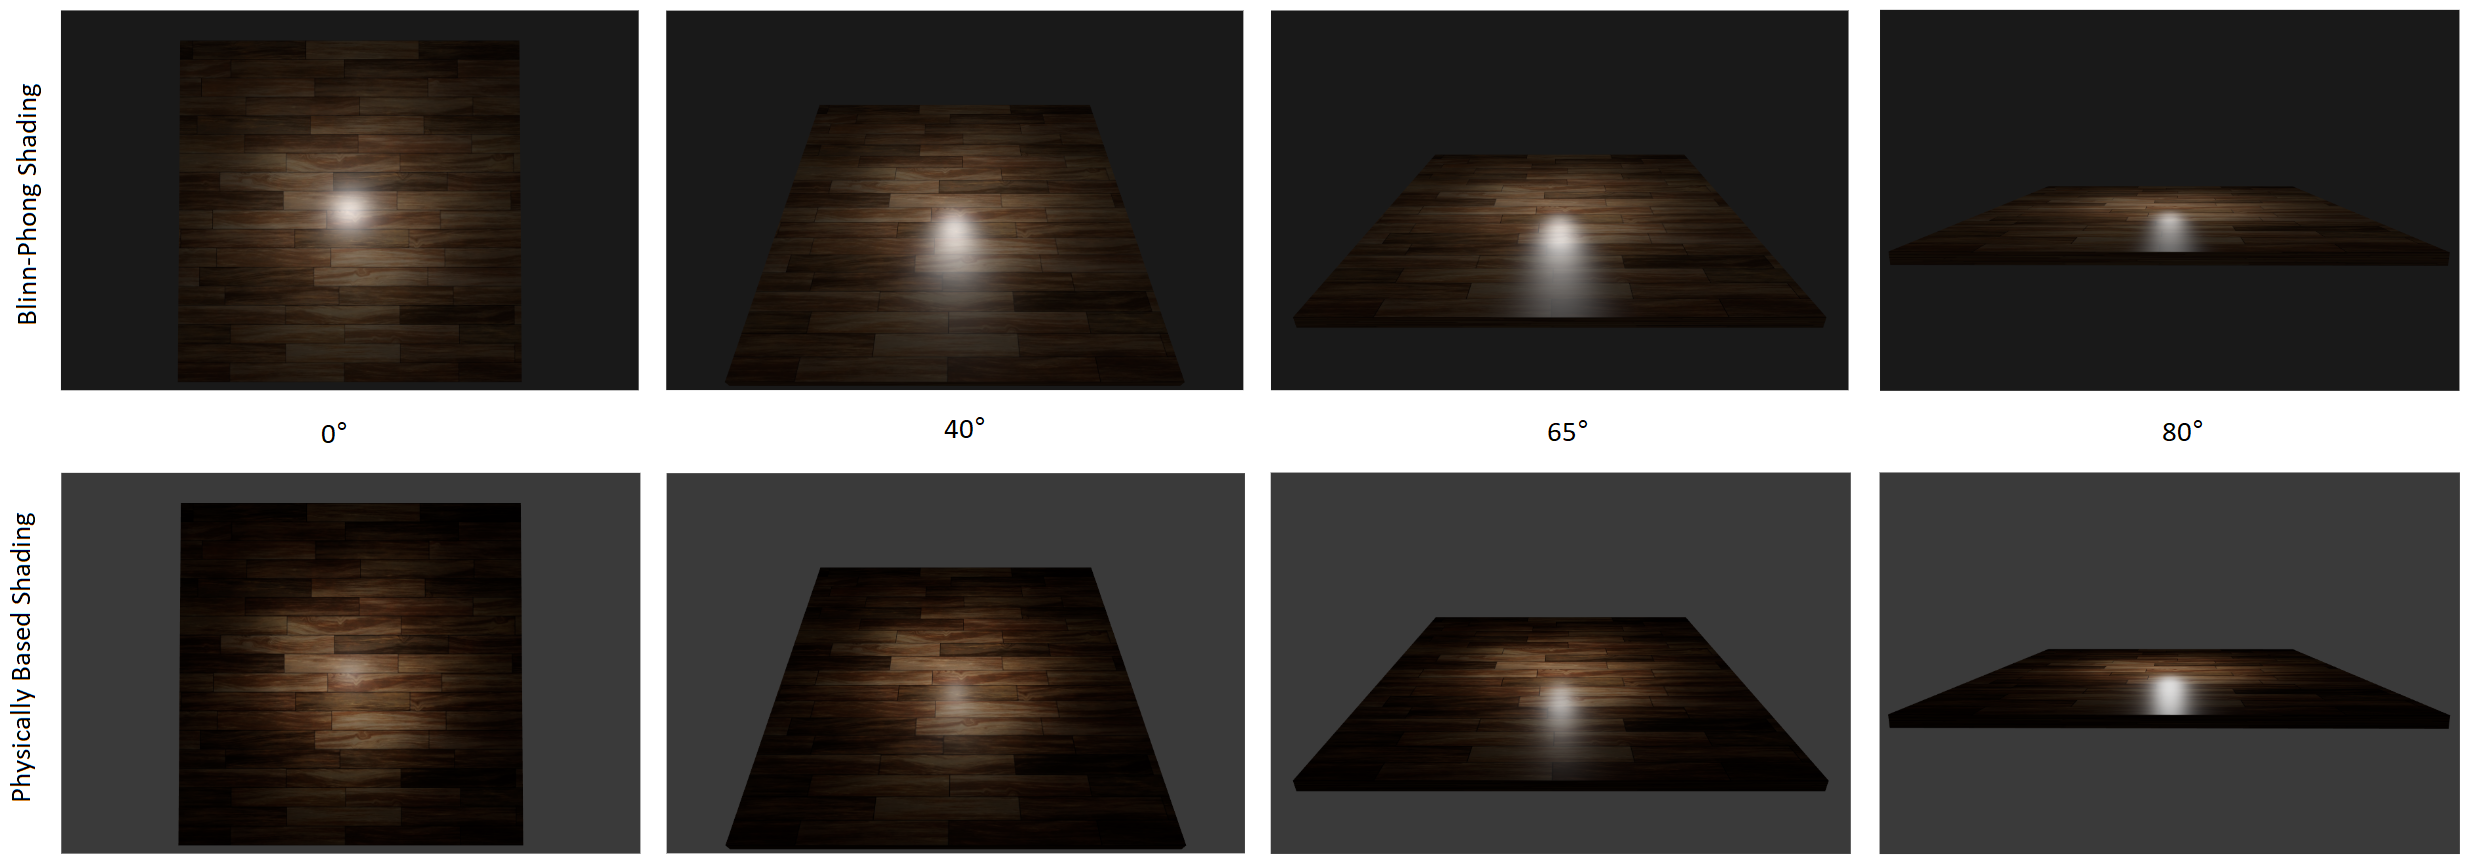
\includegraphics[width=18cm]{FresnelResults}
	\caption{Comparing Blinn-Phong and Physically Based Shading for the presence of the Fresnel effect.}
	\label{fig:FresnelResults}
\end{figure}

\subsection{Analysis}

In the frames rendered by the Blinn-Phong shading model, the wooden floor has a constant specular response over all viewing angles - the Fresnel effect is not being modelled. This is expected, as the Blinn-Phong shading model laid out in equation \ref{eq:BlinnPhong} contains no means of computing the Fresnel reflectance. This poses an issue for artists. They could choose material properties that ensure the specular response of an object is accurate at large viewing angles, but this would have the downside of making the object appear much too specular at smaller viewing angles. This was the approache used for the Blinn-Phong wooden floor material in Figure \ref{fig:FresnelResults}. Alternatively, they could do the opposite, and have more accurate specularity at smaller viewing angles, but sacrifice it at large viewing angles. Either way, a compromise is made that limits the realism of frames rendered using the Blinn-Phong shading model.

In contrast, the physically based shading model is clearly exhibiting the Fresnel effect. At small viewing angles, the wooden floor appears mostly diffuse with only a small specular response. As the angle increases towards \begin{math}90^{\circ}\end{math}, so does the specularity increase. Not only this, but the increase also follows the non-linear behaviour described in section \ref{FresnelReflectance}. This is evidenced by the fact that the specularity does not change between viewing angles \begin{math}0^{\circ}\end{math} and \begin{math}40^{\circ}\end{math}. It is at \begin{math}65^{\circ}\end{math}, and especially \begin{math}80^{\circ}\end{math}, where an increased specular response is observed. The way in which the specular response varies over the PBS frames bears close resemblance to Figure \ref{fig:FresnelRealLife}. The presence of the Fresnel effect is due to the Fresnel reflectance function in equation \ref{eq:SpecularBRDF}, which is implemented in the physically based shading model by means of the Schlick approximation.

The Fresnel effect is a physical phenomena that is accurately modelled in frames rendered by the physically based shading model, and is completely absent in frames rendered by the Blinn-Phong shading model.

\section{HDR / Energy Conservation / Long Tails?}

[Increase light power over a certian range]
[Comment on the fact that Blinn-Phong doesn't increase in brightness beyond a certian point as it just goes to white - this is because of the clipping due to non-HDR framebuffer values]
[Now dive into why the conversion between real world physical light properties to Blinn-Phong lights is not even really defined - how did I do it?]

\subsection{Testing Method}

\subsection{Results}

\subsection{Analysis}

\section{Real Time}

\begin{itemize}
	\item How it's tested
	\begin{itemize}
		\item Perhaps increasing complexities of scenes
	\end{itemize}
	\item Results of those tests (table of frame times)
	\item Discussion of results
\end{itemize}

\subsection{Testing Method}

\subsection{Results}

\subsection{Analysis}

\section{How does the industry compare scenes / evaluate shading models?}

[Frostbite has some good stuff on this]
[Disney have stuff on the MERL database - and there are lots of papers]

\subsubsection{HDR? Energy Conservation?}

<Results, evaluation (including user evaluation) {\em etc.} should be described in one or more chapters. See the `Results and Discussion' criterion in the mark scheme for the sorts of material that may be included here.>

Fresnel effect shown; energy conservation shown; more artist options shown; show the specular lobe is more accurate using PBR approaches (page 338 of the real-time rendering book)? Take pictures from papers - reconstruct scene and show how PBR is close to the paper image and Blinn-Phong isn't.
